\chapter{Introducci\'on}

En Computer Graphics, la tecnica del shading permite mejorar la percepcion de
los volumenes en 3D. Con el aumento de la capacidad de computacion estas tenicas
han evolucionado mucho en un breve periodo de tiempo.\sidenote{Is this correct?}\sidenote{I'm unsure about also!}

Las primeras aportaciones el campo fueron durante los anhos 70 por parte de Bui
Tuong Phong, Henri Gouroud y Jim Blinn con sus modelos de shading: Phong\autocite{phong}, Gouraud\autocite{gouraud}
y Blinn-Phong\autocite{blinnphong}. Estos algoritmos permiten, a partir de la posicion de la luz, y la
position de la camara, dar una estimacion de la cantidad de luz emitida por una
superficie.
\singlespacing


\begin{figure}[H]
    \setlength{\fboxsep}{0pt}
    \fbox{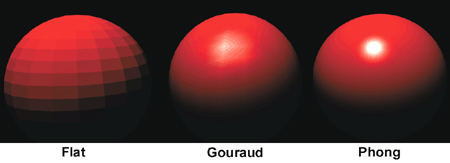
\includegraphics[width=0.99\linewidth]{images/gouroud-phong-flat.jpg}}
    \caption{A boat.}
    \singlespacing
\end{figure}

\todo[inline]{
    TODO: hablar sobre matriz de perspectiva de
    \href{http://www.cs.uns.edu.ar/cg/clasespdf/p465carlbom.pdf}
    {Ingrid Carlbon}
}

\todo[inline]{
    Siguientes a\~nos: antialising, sombras, multinucleo aparicion GPUs,
    raytracing...
    \href{https://ohiostate.pressbooks.pub/graphicshistory/back-matter/cg-historical-timeline/\#1970}
    {fuente}
}

\todo[inline]{
    Blinn’s law: “as technology advances, rendering time remains constant.” 
    from
    \href{http://www.pbr-book.org/3ed-2018/Introduction/A_Brief_History_of_Physically_Based_Rendering.html}
    {here}
}

\todo[inline]{
    Blinn's law: James Blinn first pointed out, in animation, rendering time remains
    constant, even as computers get faster. An artist gets accustomed to waiting a
    certain number of hours for an image to render, so as hardware improves, instead
    of using it to save time, he employs it to render more complex graphics. from
    \href{https://nevalalee.wordpress.com/2011/08/09/blinns-law-and-the-paradox-of-efficiency/}
    {here}
}

\todo[inline]{
    TODO: Esquema evolucion en el tiempo del shading: phong, blinn-phong
}

